\section{Auswertung}
Im Folgenden werden die Berechnungen der einzelnen Größen durchgeführt, wobei die jeweils bereits genannten Fehler aus der Versuchdurchführung zu einer
Gaußschen Fehlerfortpflanzung führen. 

\subsection{Wheatstonesche Brücke}
In dem Abschnitt \ref{sec:weedyo} sind die relevanten Fehler der gemessenen Größen aus Tabelle \ref{tab:weed} angegeben. Diese fehlerbehafteten Größen lassen sich nun in die Berechnungsgleichung ...
für den ohmschen Widerstand $R$ einsetzen.
Da hier zwei Messungen mit verschiedenen Referenzwiderständen $R_{2}$ durchgeführt wurden, ergeben sich folgende zwei Resultate.
\begin{align}
R_{10\text{,}1} &= \SI{236.5(13)}{\ohm} \\
R_{10\text{,}2} &= \SI{233.3(13)}{\ohm} 
\end{align}
Daraus lässt sich der folgende Mittelwert bestimmen, wobei sich der Fehler mittels Gaußscher Fehlerfortpflanzung ergibt.
\begin{equation}
R_{10} = \SI{234.9(9)}{\ohm}
\end{equation}
Die Fehlerfortpflanzung sieht folgendermaßen aus.
\begin{equation}
\increment R_{10} = \frac{1}{2} \sqrt{(\increment R_{10\text{,}1})^{2} + (\increment R_{10\text{,}2})^{2} }
\end{equation}


\subsection{Wien-Robinson-Brücke}

\begin{figure}
    \centering
    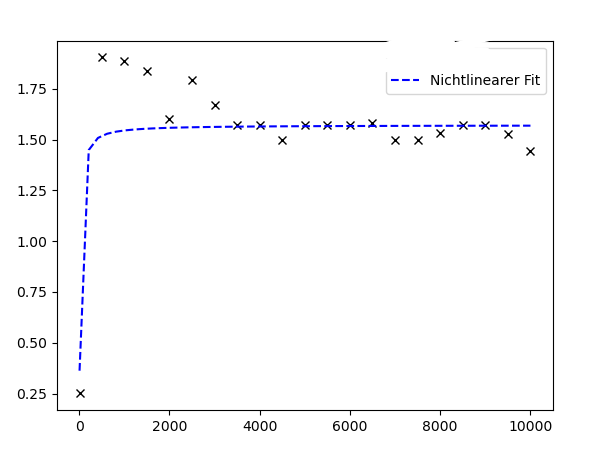
\includegraphics[width=\textwidth]{build/plot1.pdf}
    \caption{Messwerte und Theoriekurve der frequenzabhängigen Brückenspannung.} 
    \label{fig:plot1}
\end{figure}